\documentclass[border=12pt]{standalone}
\usepackage{tikz}
\usepackage{amsmath}
\usetikzlibrary{positioning,arrows.meta,fit,backgrounds,calc}
\begin{document}
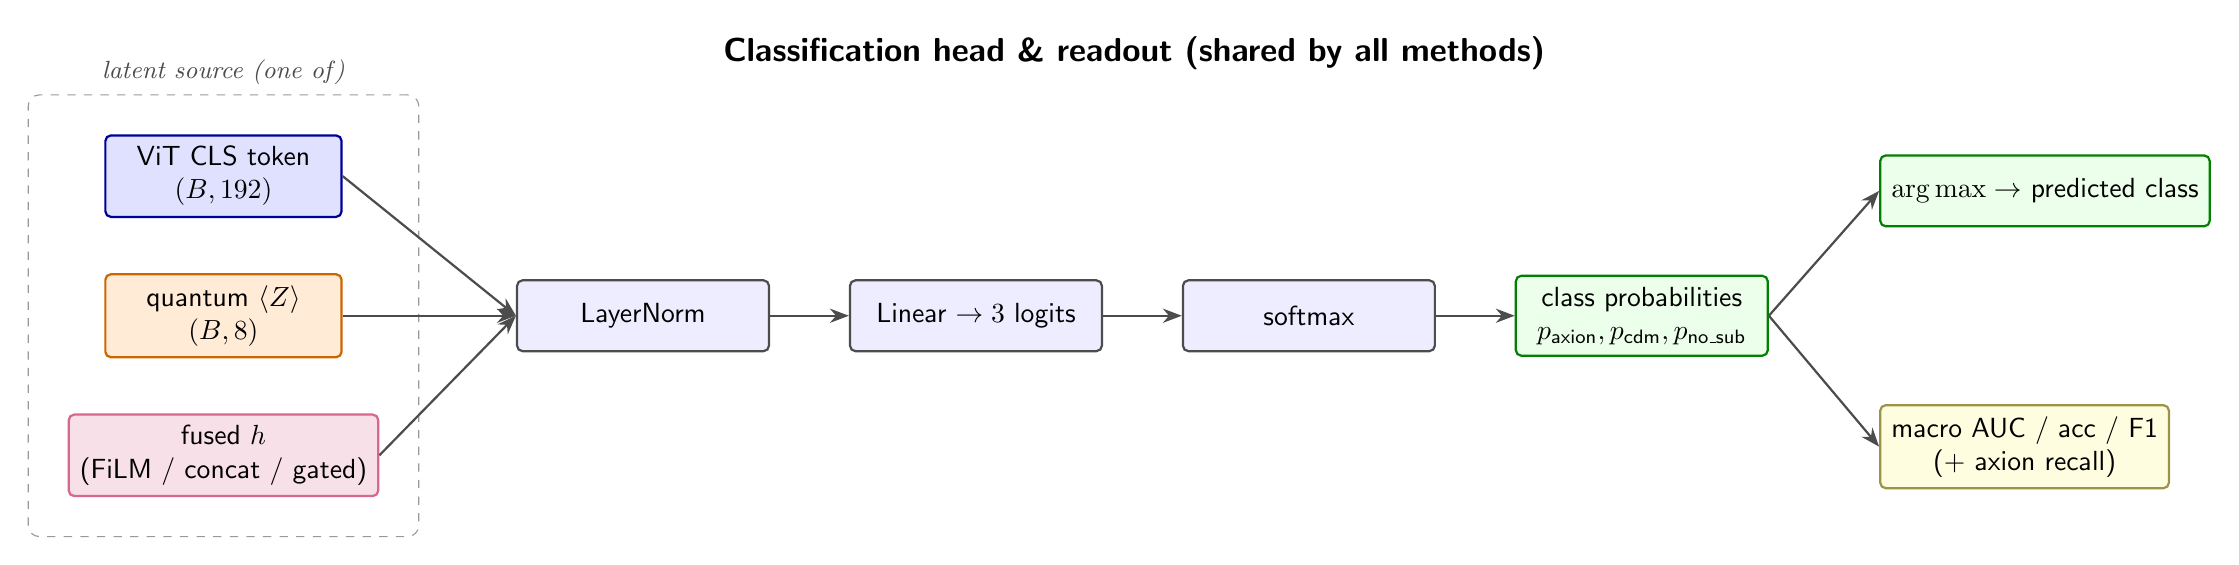
\begin{tikzpicture}[
  font=\sffamily,
  node distance=10mm,
  box/.style={rectangle,rounded corners=2pt,draw=black!70,thick,fill=blue!7,
              minimum height=9mm,minimum width=32mm,align=center,inner sep=4pt},
  src/.style={box,minimum width=30mm},
  cls/.style={box,fill=green!8,draw=green!50!black},
  metric/.style={box,fill=yellow!12,draw=yellow!55!black,minimum width=28mm},
  arr/.style={-{Stealth[length=2.4mm]},thick,black!70},
]
% three possible latent sources (left column), vertically spaced to avoid overlap
\node[src,fill=blue!12,draw=blue!60!black]                 (s1) {ViT CLS token\\$(B,192)$};
\node[src,fill=orange!16,draw=orange!80!black,below=7mm of s1] (s2) {quantum $\langle Z\rangle$\\$(B,8)$};
\node[src,fill=purple!12,draw=purple!60,below=7mm of s2]    (s3) {fused $h$\\(FiLM / concat / gated)};

\node[draw=black!40,dashed,rounded corners,fit=(s1)(s2)(s3),inner sep=5mm,
      label={[font=\small\itshape,gray!60!black]above:latent source (one of)}] (srcbox) {};

% shared readout chain (right)
\node[box,right=22mm of s2] (ln) {LayerNorm};
\node[box,right=of ln] (lin) {Linear $\to 3$ logits};
\node[box,right=of lin] (sm) {softmax};
\node[cls,right=of sm] (prob) {class probabilities\\$p_{\text{axion}},p_{\text{cdm}},p_{\text{no\_sub}}$};

\draw[arr] (s1.east) -- (ln.west);
\draw[arr] (s2.east) -- (ln.west);
\draw[arr] (s3.east) -- (ln.west);
\draw[arr] (ln)--(lin); \draw[arr] (lin)--(sm); \draw[arr] (sm)--(prob);

% two outputs from probabilities, separated vertically
\node[cls,above right=6mm and 14mm of prob] (pred) {$\arg\max\to$ predicted class};
\node[metric,below right=6mm and 14mm of prob] (auc) {macro AUC / acc / F1\\(+ axion recall)};
\draw[arr] (prob.east) -- (pred.west);
\draw[arr] (prob.east) -- (auc.west);

\node[font=\sffamily\large\bfseries]
  at ($(srcbox.north)!0.5!(pred.north)+(0,9mm)$)
  {Classification head \& readout (shared by all methods)};
\end{tikzpicture}
\end{document}
